\documentclass{beamer}

%\usetheme[framenumber,totalframenumber]{UniversiteitGent}
%\usetheme[faculty=di,framenumber,totalframenumber]{UniversiteitGent}
%\usetheme[faculty=we,usecolors,framenumber,totalframenumber]{UniversiteitGent}
\usetheme[language=english,framenumber,totalframenumber]{AlleghenyCollege}

\title{Introduction to Computer Science I}
\subtitle{\textcolor{black}{Introduction to Programming}}
\author{Janyl Jumadinova \\ 22-24 January, 2018}

\begin{document}

\begin{frame}
  \titlepage
\end{frame}

%%%%%%%%%%%% Slide %%%%%%%%%%%%%%%%%%%%%%%%%%%%%%%%%%%%%%%%%%%%%%%%%%%
\begin{frame}
  \frametitle{What is Computer Science?}
	\begin{itemize}
		\item A \textcolor{blue}{computation} is a sequence of well-defined operations that lead from an initial starting point to a desired final outcome
    \end{itemize}
    \pause
    \begin{block}{\centering \Large{Computer science is the study of computation}}
    \end{block}
\end{frame}
%%%%%%%%%%%% Slide %%%%%%%%%%%%%%%%%%%%%%%%%%%%%%%%%%%%%%%%%%%%%%%%%%%
\begin{frame}
  \frametitle{}
  Computer science is the study of computation
  \pause
  	\begin{itemize}
		\item investigating problems that can be solved computationally \pause
		\item programming languages used to describe computations \pause
		\item machines that carry out computations \pause
		\item theoretical limits of computation (what is or is not computable) \pause
		\item \textbf{computational solutions to problems in math, science, medicine,  business, education, journalism, ...} \pause
    \end{itemize}
    
Computers play a key role
\end{frame}

%%%%%%%%%%%% Slide %%%%%%%%%%%%%%%%%%%%%%%%%%%%%%%%%%%%%%%%%%%%%%%%%%%
\begin{frame}
  \frametitle{Applications of Computer Science}
  Motion Analysis
  \begin{center}
  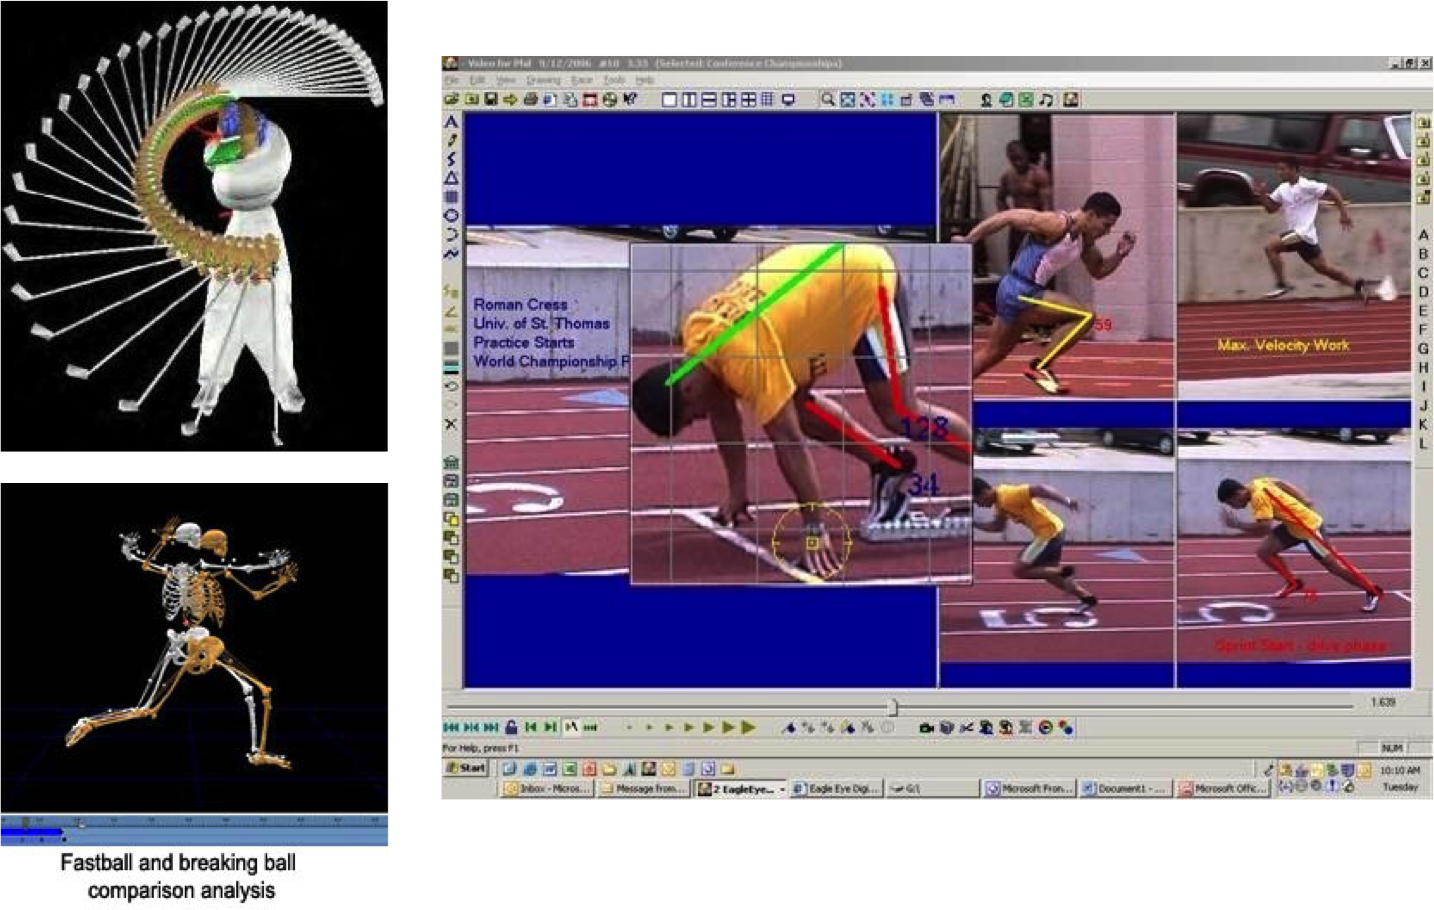
\includegraphics[scale=0.35]{images/sports}
  \end{center}
\end{frame}
%%%%%%%%%%%% Slide %%%%%%%%%%%%%%%%%%%%%%%%%%%%%%%%%%%%%%%%%%%%%%%%%%%
\begin{frame}
  \frametitle{Applications of Computer Science}
  Animated Movies ... 
  \begin{center}
  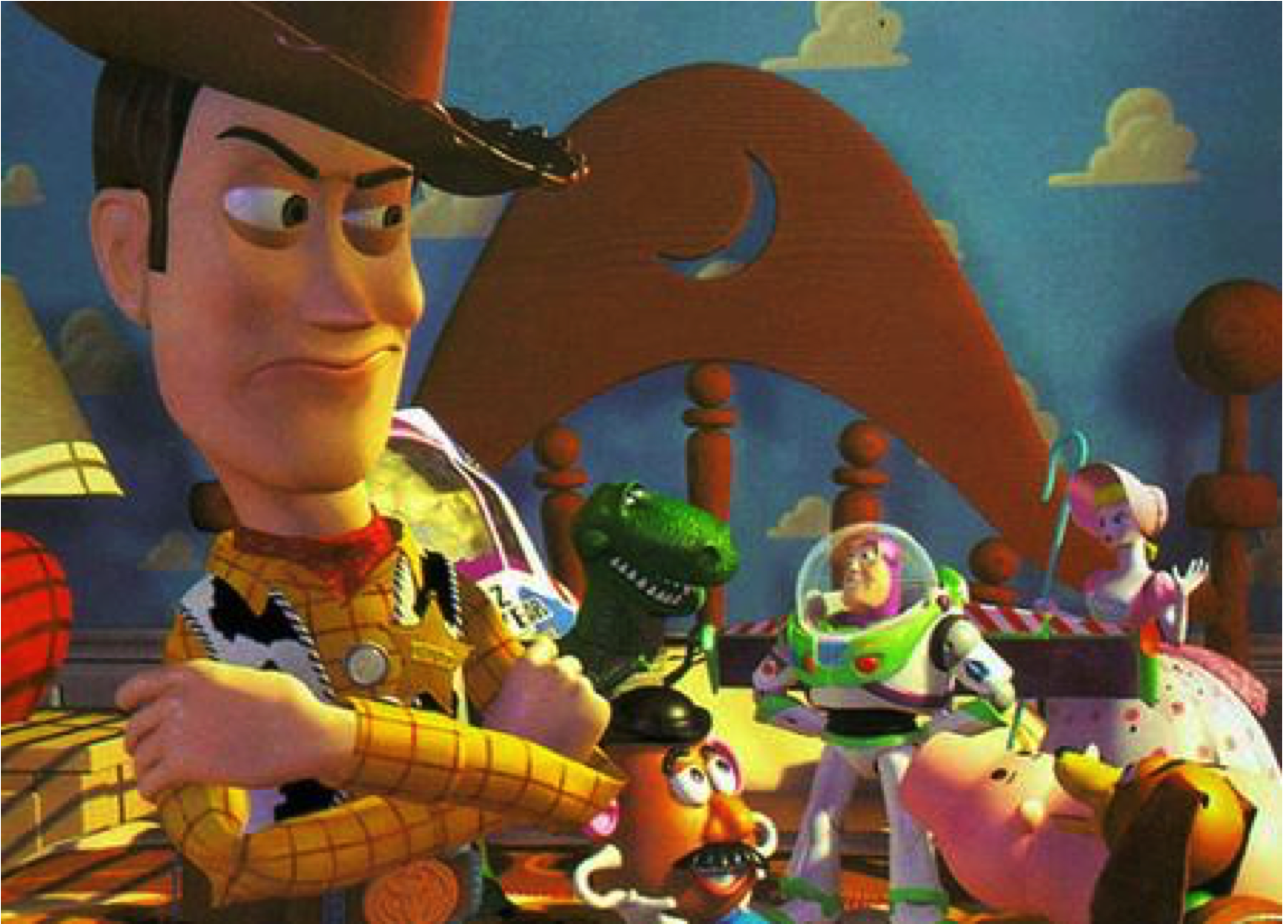
\includegraphics[scale=0.3]{images/ani1}
  \end{center}
\end{frame}
%%%%%%%%%%%% Slide %%%%%%%%%%%%%%%%%%%%%%%%%%%%%%%%%%%%%%%%%%%%%%%%%%%
\begin{frame}
  \frametitle{Applications of Computer Science}
  ... are made by Computer Scientists
  \begin{center}
  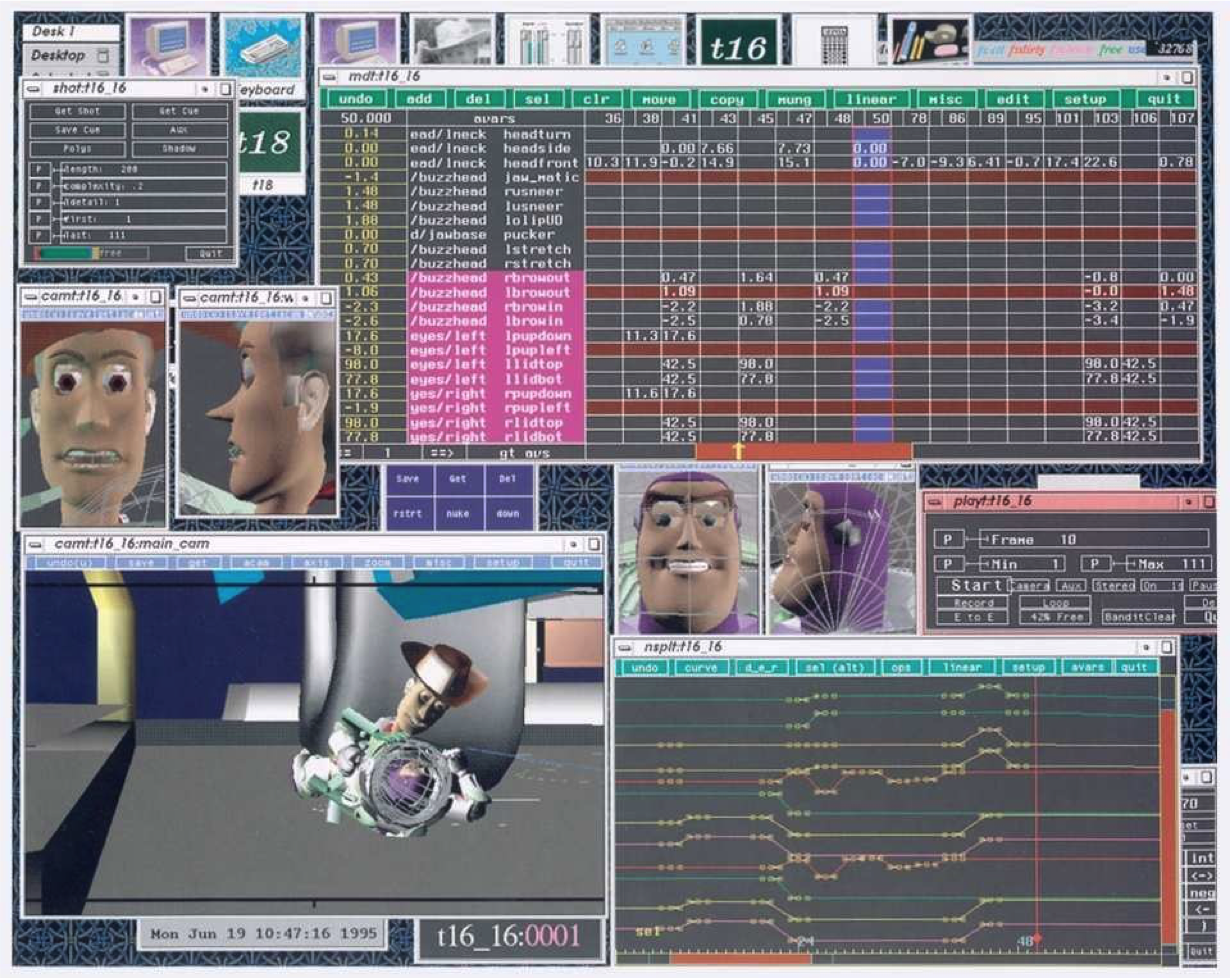
\includegraphics[scale=0.3]{images/ani2}
  \end{center}
\end{frame}
%%%%%%%%%%%% Slide %%%%%%%%%%%%%%%%%%%%%%%%%%%%%%%%%%%%%%%%%%%%%%%%%%%
\begin{frame}
  \frametitle{Applications of Computer Science}
  \begin{center}
  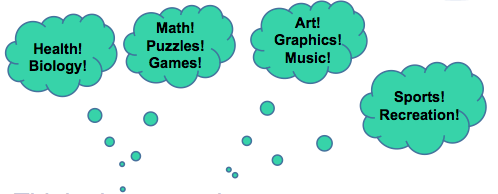
\includegraphics[scale=0.5]{images/interests}
  \end{center}
  \begin{itemize}
  	\item Think about your interests ...
	\item You can bet computer scientists are working in these areas!
  \end{itemize}
\end{frame}
%%%%%%%%%%%% Slide %%%%%%%%%%%%%%%%%%%%%%%%%%%%%%%%%%%%%%%%%%%%%%%%%%%
\begin{frame}
  \frametitle{What is a computer?}
     \begin{center}
        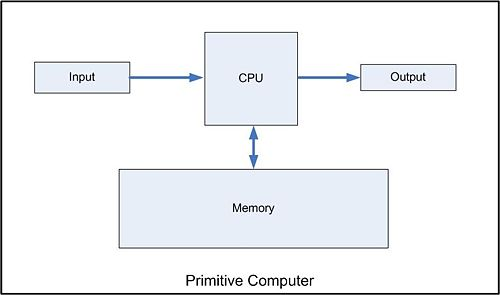
\includegraphics[width=3in]{images/simple.jpg}
    \end{center}
\end{frame}
%%%%%%%%%%%% Slide %%%%%%%%%%%%%%%%%%%%%%%%%%%%%%%%%%%%%%%%%%%%%%%%%%%
\begin{frame}
  \frametitle{Hardware/Software}
	\begin{itemize}
        \item Software/hardware relationship:
        \begin{itemize}
			\item Hardware is controlled by software
			\item Software is the collection of instructions that you issue to the computer to perform actions and make decisions
		\end{itemize}
    \end{itemize}
\end{frame}
%%%%%%%%%%%% Slide %%%%%%%%%%%%%%%%%%%%%%%%%%%%%%%%%%%%%%%%%%%%%%%%%%%
\begin{frame}
  \frametitle{Simple Structure}

        \begin{center}
        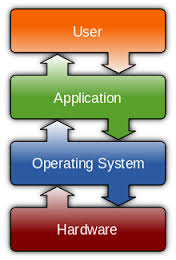
\includegraphics[width=1.5in]{images/structure.jpeg}
    \end{center}
\end{frame}
%%%%%%%%%%%% Slide %%%%%%%%%%%%%%%%%%%%%%%%%%%%%%%%%%%%%%%%%%%%%%%%%%%

\begin{frame}
  \frametitle{What is Computer Programming?}
		\pause
      \begin{itemize}
        \item Programming is the act of writing usable and useful software
        \item A program is a set of instructions
    \end{itemize}
\end{frame}

%%%%%%%%%%%% Slide %%%%%%%%%%%%%%%%%%%%%%%%%%%%%%%%%%%%%%%%%%%%%%%%%%%
\begin{frame}
  \frametitle{Programming Language}
	\begin{itemize}
		\item We will use \textbf{Java} programming language in this class
		\item Java is a programming language originally developed by Sun Microsystems and released in 1995 as a core component of Sun's Java platform
    \end{itemize}
\end{frame}

%%%%%%%%%%%% Slide %%%%%%%%%%%%%%%%%%%%%%%%%%%%%%%%%%%%%%%%%%%%%%%%%%%
\begin{frame}
  \frametitle{HISTORY OF JAVA}
    \begin{itemize}
        \item Started development in 1991 at Sun
		\item Originally called Oak
		\item Intended for smart consumer-electronic devices
		\item Derives much syntax/concepts from C++
		\item BCPL $\rightarrow$ B $\rightarrow$ C $\rightarrow$ C++ $\rightarrow$ Java
		\item Development almost halted, but 1993 saw introduction of web; Java was revamped to be able to easily add dynamic content to web pages
		\item Formally announced and released in May 1995
		\item Released under GPL to the public in May 2007
    \end{itemize}

\end{frame}

%%%%%%%%%%%% Slide %%%%%%%%%%%%%%%%%%%%%%%%%%%%%%%%%%%%%%%%%%%%%%%%%%%
\begin{frame}
  \frametitle{Programming in Java}
	\begin{itemize}
		\item Java is an \textcolor{blue}{object-oriented} programming language \pause
		\item \textcolor{blue}{Objects} are fundamental elements that make up a program \pause
		\item Java has a library of software, called \textcolor{blue}{Java API}, that is available for your use
    \end{itemize}
\end{frame}
%%%%%%%%%%%% Slide %%%%%%%%%%%%%%%%%%%%%%%%%%%%%%%%%%%%%%%%%%%%%%%%%%%
\begin{frame}
  \frametitle{Java program development process}
		 \begin{center}
    			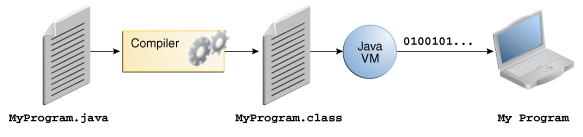
\includegraphics[scale=0.55]{images/compilation}
    		 \end{center}
\end{frame}
%%%%%%%%%%%% Slide %%%%%%%%%%%%%%%%%%%%%%%%%%%%%%%%%%%%%%%%%%%%%%%%%%%
\begin{frame}[fragile]
  \frametitle{Simple first Java Program: ``Hello World''}
  \vspace{-0.1in}
  {\small{
\begin{verbatim}
// This is the first program people write in a new language, 
// the "Hello World!".  In Java, this file must be named 
// Welcome.java, with the first part of the name, Welcome, being 
// the same as the name of the class. The filename itself 
// (not the class name) must always end in .java to indicate
// to the operating system that it's a java source file.
public class Welcome
{
 	public static void main ( String args[] )
 	{
 	    System.out.println ( "Hello World!" );
 	}
 }
\end{verbatim}
}}
\end{frame}
%%%%%%%%%%%% Slide %%%%%%%%%%%%%%%%%%%%%%%%%%%%%%%%%%%%%%%%%%%%%%%%%%%
\begin{frame}
  \frametitle{Comments}
  Comments in Java can be one of three styles:
	\begin{itemize}
		\item \textbf{Single line:} starts at // anywhere on a line, ends at the end of that line
		\item \textbf{Multi-line:} starts with character sequence /* anywhere, ends with character sequence */ anywhere after that can span multiple lines
		\item \textbf{javadoc:} starts with character sequence /** anywhere, ends with character sequence */ anywhere, after that uses javadoc utility to create HTML documentation from code
    \end{itemize}
\end{frame}
%%%%%%%%%%%% Slide %%%%%%%%%%%%%%%%%%%%%%%%%%%%%%%%%%%%%%%%%%%%%%%%%%%
\begin{frame}
  \frametitle{}
  	\begin{itemize}
		\item \textcolor{brown}{public class Welcome}: 
		\begin{itemize}
		\item \textbf{public} means that something is available across packages (reserved word)
		\item Name of the class has to be the same as the name of the .java file 
		\end{itemize}
		\pause
		\item \textcolor{brown}{public static void main ( String \textcolor{blue}{identifier}[] )}: \\
		\begin{itemize}
		\item The particular form of main is required by Java.
		\item JVM starts executing here! 
		\item main is a static method, it is part of its class and not part of objects. 
		\item Strings in Java are sequence of characters	
		\end{itemize}
		\pause
		\item Braces \{   \} are used to collect statements into a "block" 
		\pause
		\item Statements in Java end with semicolons. 
    \end{itemize}
\end{frame}
%%%%%%%%%%%% Slide %%%%%%%%%%%%%%%%%%%%%%%%%%%%%%%%%%%%%%%%%%%%%%%%%%%
\begin{frame}
  \frametitle{Printing}
  \begin{itemize}
		\item \textcolor{brown}{println:} New line after printing
		\item \textcolor{brown}{print:} No new line
		\item \textcolor{brown}{printf:} Can specify format - may learn this later
    \end{itemize}
\end{frame}

%%%%%%%%%%%% Slide %%%%%%%%%%%%%%%%%%%%%%%%%%%%%%%%%%%%%%%%%%%%%%%%%%%
\begin{frame}
  \frametitle{Character Strings}
  \begin{block}{string literal in class \textcolor{brown}{String}}
  ``ABC'' \\ 
  ``This is interesting''\\
  `` '' \\
  ``91''
  \end{block}
  \pause
\begin{itemize}
	\item Use \textcolor{blue}{print} or \textcolor{blue}{println} methods to print a character string to the terminal
	\item \textcolor{blue}{System.out.println(``CMPSC 111");}
	\item the string \textcolor{blue}{``CMPSC 111"} is a \textcolor{red}{parameter}: data sent to a method
\end{itemize}
\end{frame}
%%%%%%%%%%%% Slide %%%%%%%%%%%%%%%%%%%%%%%%%%%%%%%%%%%%%%%%%%%%%%%%%%%
\begin{frame}
  \frametitle{String Concatenation}
  \begin{block}{appending one string to the end of another: use + operator}
  ``This is ''+ ``interesting''\\
  ``Your grade is ''+ ``91''
  \end{block}
  \pause
\begin{itemize}
	\item + is also used for arithmetic addition
	\item \textcolor{blue}{System.out.println("Adding "+ 12 + 23);} is not the same as \textcolor{blue}{System.out.println("Adding "+ (12 + 23));}
\end{itemize}
\end{frame}
%%%%%%%%%%%% Slide %%%%%%%%%%%%%%%%%%%%%%%%%%%%%%%%%%%%%%%%%%%%%%%%%%%
\begin{frame}[fragile]
  \frametitle{Escape Sequences}
	\begin{itemize}
		\item Escape sequences, or escape characters, begin with a slash and are immediately followed by another character.  
		\item This two-character sequence, inside `` '' allows you to control your output (\textbackslash n, \textbackslash t, \textbackslash b) or output characters you wouldn't otherwise be able to (\textbackslash\textbackslash, \textbackslash ") inside a string.
    \end{itemize}
\end{frame}
%%%%%%%%%%%% Slide %%%%%%%%%%%%%%%%%%%%%%%%%%%%%%%%%%%%%%%%%%%%%%%%%%%
\begin{frame}[fragile]
  \frametitle{Escape Sequences}
\begin{tabular}{|c|c|c|}
\hline
Seq &	Meaning	&	    Example Code \\
\hline
\textbackslash n	& New line		&    System.out.println("Hi\textbackslash nThere"); \\

\textbackslash t	&Horizontal tab	& System.out.println("What's\textbackslash tup?"); \\

\textbackslash b &	Backspace	  &  System.out.println("Hi\textbackslash b Hey"); \\

\textbackslash\textbackslash &	Backslash	 &   System.out.println("Back\textbackslash\textbackslash Slash"); \\

\textbackslash "	 &Double quote	&    System.out.println("Dbl\textbackslash "Quote"); \\
\hline
\end{tabular}

\end{frame}

%%%%%%%%%%%% Slide %%%%%%%%%%%%%%%%%%%%%%%%%%%%%%%%%%%%%%%%%%%%%%%%%%%
\end{document}
